%% Author_tex.tex
%% V1.0
%% 2012/13/12
%% developed by Techset
%%
%% This file describes the coding for rstrans.cls

\documentclass[openacc]{rstransa}%%%%where rstrans is the template name

%%%% *** Do not adjust lengths that control margins, column widths, etc. ***

%%%%%%%%%%% Defining Enunciations  %%%%%%%%%%%
\newtheorem{theorem}{\bf Theorem}[section]
\newtheorem{condition}{\bf Condition}[section]
\newtheorem{corollary}{\bf Corollary}[section]
%%%%%%%%%%%%%%%%%%%%%%%%%%%%%%%%%%%%%%%%%%%%%%%
\newcommand{\Reyn}{\mathrm{Re}}
\newcommand{\Lop}{\mathcal{L}}
\begin{document}

%%%% Article title to be placed here
\title{Generalized Quasi-linear Approximation and Non-normality in Taylor-Couette Flow}

\author{%%%% Author details
Jeffrey S. Oishi and Morgan Baxter}

%%%%%%%%% Insert author address here
\address{Department of Physics and Astronomy, Bates College, Lewiston, ME USA}

%%%% Subject entries to be placed here %%%%
\subject{xxxxx, xxxxx, xxxx}

%%%% Keyword entries to be placed here %%%%
\keywords{xxxx, xxxx, xxxx}

%%%% Insert corresponding author and its email address}
\corres{Jeffrey S. Oishi\\
\email{joishi@bates.edu}}

%%%% Abstract text to be placed here %%%%%%%%%%%%
\begin{abstract}
Taylor-Couette flow is well known to admit a spiral turbulence state in which laminar and turbulent patches coexist around the cylinder. This flow state is quite complex, with delicate internal structure, and it can be traced into certain regimes of linear stability. This behavior is believed to be connected to the non-normality of the linear operator, which is itself a function of the control parameters. Using spiral turbulence in both linearly stable and unstable regimes, we investigate the effectiveness of the generalized quasilinear approximation (GQL), an extension of quasilinear theory designed to capture the essential aspects of turbulent flows. We find that GQL performs much better in the supercritical regime than the subcritical. By including only a small number of modes into the non-linear interactions, GQL simulations maintain a turbulent-like state when in the supercritical regime. However, a much larger number is required to avoid returning to the laminar state when in the subcritical regime. 
\end{abstract}
%%%%%%%%%%%%%%%%%%%%%%%%%%%

%%%%%%%%%% Insert the texts which can accomdate on firstpage in the tag "fmtext" %%%%%

%\begin{fmtext}
%\end{fmtext}
%%%%%%%%%%%%%%% End of first page %%%%%%%%%%%%%%%%%%%%%

\maketitle

\section{Introduction}
\label{sec:intro}
%Something about Taylor (1923); GQL.
Since Taylor's classic 1923 paper\cite{1923RSPTA.223..289T}, fluid between two independently rotating cylinders has become a rich laboratory for the understanding of instability, transition to turbulence, and turbulence itself. Indeed, the interplay between experiment, computation, and theoretical understanding evinced in Taylor's paper remains a model for the study of fluid dynamics.

Some of the most common forms of turbulence in nature are anisotropic, with a symmetry broken by rotation, magnetic fields, or boundary effects. In these situations, significant theoretical progress can be made by considering \emph{quasi-linear} (QL) models, in which one retains only those non-linearities that contribute to the mean flow. Recently, the generalized quasi-linear approximation (GQL) has been developed to systematically expand the QL idea to include sets of non-linear interactions between two \emph{sets} of modes, low and high, respectively, discarding those that involve only high modes (see \cite{2022arXiv220505513M} for a recent review). GQL has been shown to perform significantly better in reproducing direct numerical simulations (DNS) than QL models across a wide range of paradigm flows including forced zonal jet formation \cite{2016PhRvL.116u4501M}, rotating plane Couette flow \cite{2017JFM...810..412T}, rapidly rotating convection \cite{2018RSPSA.47480422T}, and channel flow\cite{2019Kellam}.

Here, we consider Taylor-Couette (TC) flows at moderate inner and outer Reynolds numbers, $|\Reyn_{i,o}| < 3500$. This is an interesting testbed for GQL because it features numerous intricate patterns that are maintained by non-linear interactions beyond the cascade, local in coefficient space, found at high $\Reyn$. 
One of the key feature of TC flow is that it has non-linear and linear instabilities in different regions of parameter space. In the linearly stable regions, transient growth has been observed in TC flow\cite{2002PhFl...14.3475H, 2002PhFl...14.1655M}. 
We can always write the Navier-Stokes equations in schematic form as
\begin{equation}
    \label{eqn:NS-schematic}
    \frac{\partial \mathbf{q}}{\partial t} + \Lop \mathbf{q} = \mathcal{N}(\mathbf{q}),
\end{equation}
where $\Lop$ is a linear operator and $\mathcal{N}$ is a non-linear function of the state vector $\mathbf{q} = \left[ \mathbf{u}  p\right]^T$, where $\mathbf{u}$ is the velocity field and $p$ the pressure.
As noted by \cite{2002PhFl...14.3475H}, the linear operator $\Lop$ for TC flow is a function of its control parameters.
That is, its commutator with its adjoint
\begin{equation}
    [\Lop^\dagger, \Lop] = f(\mu, \eta, \Reyn_i, \Gamma)
\end{equation}
can be zero or non-zero. 
This provides a very useful arena to test the validity of GQL in a system that admits a varying degree of non-normality.

As a first experiment to this end, we consider the \emph{spiral turbulence} flow regime. The classic paper by Coles \cite{1965JFM....21..385C} was the first to note a hysteretic transition to spiral turbulence when the cylinders were counter-rotating: an experiment at fixed $\Reyn_o$ will have spiral turbulence at a certain $\Reyn_i$ if $\Reyn_i$ is reached by \emph{decreasing} from a higher value, but will not have spiral turbulence at the same $\Reyn_i$ if it is reached by \emph{increasing} from a lower value. More recent work has identified both supercritical and subcritical paths to spiral turbulence\cite{2009PhRvE..80d6315M}. In that work, the authors follow spiral turbulence along a decreasing $\Reyn_i$ path and show that the state is maintained even below the linear stability boundary when $\Reyn_o = -3000$ but it relaminarizes below the stability boundary when $\Reyn_o = -1200$.
Using \cite{2009PhRvE..80d6315M} as a guide, we use direct numerical simulations (DNS) at $\Reyn_o = -3398$ and decrease $\Reyn_i$ into the subcritical region. We then run a suite of GQL simulations in both the super- and subcritical regions.

We begin in section~\ref{sec:methods} by detailing our equations, non-dimensionalization, and numerical methods. Section~\ref{sec:linear} reviews both modal and non-modal linear analyses and contains a new analysis combining linear and non-linear aspects. In section~\ref{sec:nonlinear}, we describe the main results of the paper, the comparison of DNS, QL, and GQL in each of the three regimes. Finally, we offer discussion and concluding results in section~\ref{sec:conclusion}.
%Recently, a subcritical transition to turbulence via interpenetrating spirals has been reported \cite{2020JFM...892A..12C}. This work has a small aspect ratio $\Gamma = 5.26$, which delays the onset of linear instability to considerably higher $\Reyn_1$ for a given $\Reyn_2$. 

\section{Methods}
\label{sec:methods}
We solve the incompressible Navier-Stokes equations with unit density for $\mathbf{u}' = \mathbf{u} - \mathbf{U}$,
where $\mathbf{U} = A r + B/r \hat{\mathbf{e}}_\phi$ is circular Couette flow (CCF),
\begin{align}
\label{eqn:NS}
      \frac{\partial \mathbf{u'}}{\partial t} + \mathbf{U} \cdot \nabla \mathbf{u'} + \mathbf{u'} \cdot \nabla \mathbf{U} + \mathbf{u'} \cdot \nabla \mathbf{u'} &= -\nabla p + \nu \nabla^2\mathbf{u'}\\
      \nabla \cdot \mathbf{u'} &= 0.
\end{align}
In order to implement the GQL approximation, we introduce a projection operator to divide $\mathbf{u'}$ into two subsets,
\begin{align}
    \mathbf{u'}_l = \left< \mathbf{u'}\right>_l &= \sum_{m = -\Lambda_\theta}^{\Lambda_\theta} \sum_{k = -\Lambda_z}^{\Lambda_z} \mathbf{\hat{u}'}_{mk}(r) e^{i (m \theta + 2\pi k z/L_z)}\\
    \mathbf{u'}_h = \mathbf{u'} - \mathbf{u'}_l.
\end{align}
GQL can then be written as 
\begin{align}
\label{eqn:GQL}
      \frac{\partial \mathbf{u'}}{\partial t} + \mathbf{U} \cdot \nabla \mathbf{u'} + \mathbf{u'} \cdot \nabla \mathbf{U} +\nabla p - \nu \nabla^2\mathbf{u'} = &- \left<\mathbf{u'}_l \cdot \nabla \mathbf{u'}_l +\mathbf{u'}_h \cdot \nabla \mathbf{u'}_h\right>_l\\
      & +\left<\mathbf{u'}_l \cdot \nabla \mathbf{u'}_h + \mathbf{u'}_h \cdot \nabla \mathbf{u'}_l \right>_h\\
      \nabla \cdot \mathbf{u'} = & 0,
\end{align}
where we have written all linear terms on the left hand side. This form is equivalent to those given in prior works (for example \cite{2017JFM...810..412T}), where separate equations are written for the low and high modes, respectively.
For all runs in this paper, $\Lambda = \Lambda_z = \Lambda_\theta$, though we note it would be interesting to consider models quasilinear in $\theta$ (i.e. $\Lambda_\theta = 0$) with varying $\Lambda_z$. These correspond to the \emph{restricted non-linear} models used with success in shear flow turbulence \cite{2014PhFl...26j5112T, 2015PhFl...27j5104T, 2015PhFl...27a1702B}.

We non-dimensionalise lengths in terms of the gap width $d = R_2 - R_1$ and velocities in terms of the inner cylinder velocity $U_i = R_i \Omega_i$. Taylor-Couette flow can be parameterised in terms of four parameters, the inner cylinder Reynolds number $\Reyn_i$, the ratio of inner to outer radii $\eta \equiv R_i/R_o$, the ratio of outer to inner rotation rates $\mu \equiv \Omega_o/\Omega_i$, and the aspect ratio of the cylinder $\Gamma \equiv L_z/d$. In our computations, the $z$ direction is periodic and thus $L_z$ is the periodicity length. We will also refer to the two Reynolds numbers $\Reyn_i$, $\Reyn_o$, related by
\begin{equation}
    \frac{\Reyn_o}{\Reyn_i} = \frac{\mu}{\eta}.
\end{equation}
It is also quite useful to characterize times in terms of the viscous diffusion time $\tau_\nu \equiv d^2/\nu$. In our units, $\tau_\nu = \Reyn_i$.

We use the pseudo-spectral Dedalus framework (version 2) \cite{2020PhRvR...2b3068B} for all linear and non-linear calculations. We discretize the three velocity components and pressure onto a basis of Chebyshev polynomials in the radial direction, while $\theta$ and $z$ use Fourier bases.
To evolve the solution forward in time, we use the implicit-explicit Runga-Kutta RK443 time stepper; linear terms are implicitly timestepped while non-linear terms are explicit.
Our initial value solver has been extensively tested for TC flow against the linear and non-linear test cases in \cite{1984JFM...146...45M, 1984JFM...146...65M} including linear growth rates, non-linear wave speeds, and torque measurements; our spiral turbulence DNS results also agree with those in \cite{2009PhRvE..80d6315M,2009PhRvE..80f7301D,2011JFM...668..150D}. 
Resolutions and geometric parameters for all runs are given in table~\ref{tab:simulations}.
\begin{table}[!h]
\caption{Simulations}
\label{tab:simulations}
\begin{tabular}{rlllllllll}
\hline
$\Reyn_i$ & $\Reyn_o$ & $\eta$ & $\Gamma$  & $N_r$ & $N_\theta$ & $N_z$& $\Lambda_\theta$, $\Lambda_z$ & Notes\\
\hline
%A & 750  & 0 & 0.875  & 3 & 32 & 64 & 64 & 0, 1, 3, 5 & WVF\\
%B & 1000 & 0 & 0.875 & 3 & 32 & 256 & 64 & 0, 1, 3, 5 & MWF\\
%C & 2000 & 0 & 0.875 & 3 & 32 & 512 & 64 & 0, 1, 3, 5 & TTV\\
%\hline
900 & -3398 & 0.883 & 29.9 & 64 & 512 & 512 & 0, 1, 3, 5, 10 & Supercritical SPT\\
700 & -3398 & 0.883 & 29.9 & 64 & 512 & 512 & 0, 1, 3, 5, 10, 20, 30 & Subcritical SPT\\
%\hline
%F & 640 & -1359 & 0.883 & 29.9 & 64 & 512 & 512 & 0, 1, 3, 5 & Supercritical SPT\\
%G & 480 & -1359 & 0.883 & 29.9 & 64 & 512 & 512 & 0, 1, 5 & Supercritical IPS\\
\end{tabular}
\vspace*{-4pt}
\end{table}%%%End of the table
We have confirmed our simulations are resolved by ensuring that the highest wavenumber components have spectral power at least $10^5$ smaller than the most energetic scale.

Pseudospectra and critical parameters are calculated using eigentools \cite{2021JOSS....6.3079O}.

\section{Linear Stability}
\label{sec:linear}
In order to determine the linear stability bound, we find the minimum $\Reyn_i$ for a given $\Reyn_o$ by solving the eigenvalue problem for equations~\ref{eqn:NS}. We note that for all $\Reyn_o$ plotted in figure~\ref{fig:LSB}, most unstable mode is never axisymmetric. At $\Reyn_o=-3398$, where our non-linear calculations are run, the most unstable mode has $m = 5$ at onset, and 
\begin{figure}
    \centering
    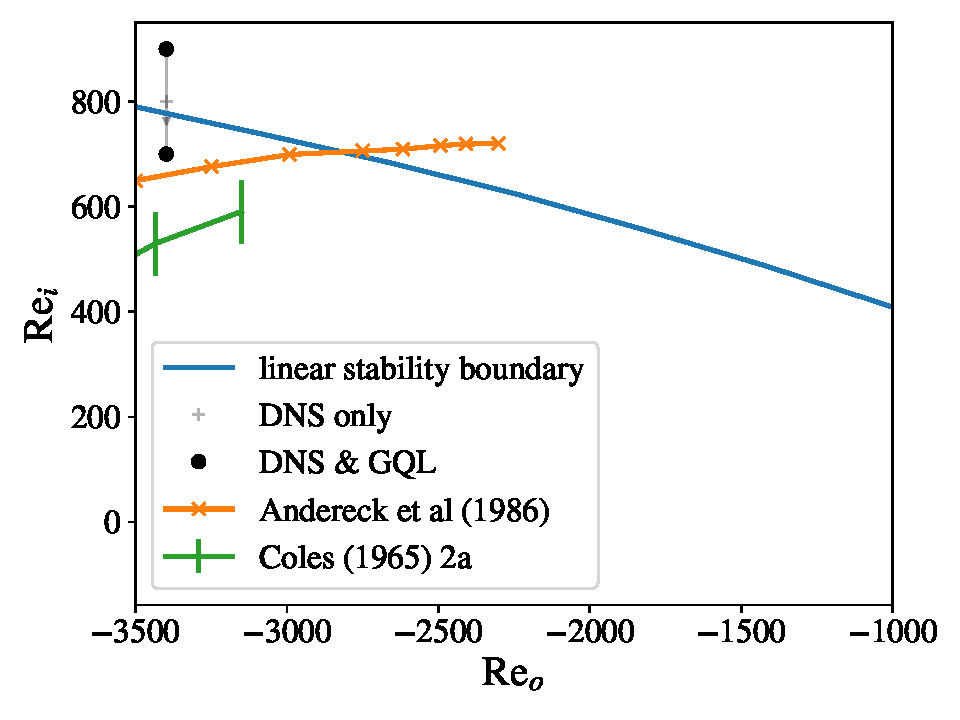
\includegraphics[width=0.8\textwidth]{../figs/reo_rei_lsb.pdf}
    \caption{A summary of spiral turbulence runs in the $\Reyn_o-\Reyn_i$ plane showing linear stability boundary. Solid circles shows points where we have conducted GQL analysis; crosses represent DNS steps along the path to subcritical behaviour. }
    \label{fig:LSB}
\end{figure}

The spiral turbulence regime provides an ideal opportunity to test GQL in an environment with both spatiotemporal patterns and a tunable bifurcation: by choosing $\Reyn_i$ and $\Reyn_o$ appropriately, both subcritical and supercritical manifestations of spiral turbulence can be selected.
Following pioneering numerical work \cite{2009PhRvE..79c6309M, 2009PhRvE..80d6315M}, we set the outer cylinder rotation rate to $\Reyn_o = -3398$ for the subcritical path and $\Reyn_o = -1359$ for the supercritical path and start a series of DNS runs at a $\Reyn_i$ high enough to trigger spiral turbulence driven by linear instability from a low-amplitude, random inital condition satisfying $\nabla \cdot \mathbf{u} = 0$.
From these two seed runs, we decrease $\Reyn_i$ in steps shown in figure~\ref{fig:LSB} where each point represents a DNS or GQL simulation run for one viscous time. The solid circles in figure~\ref{fig:LSB} represent runs where we performed GQL analyses. 

\section{Results}
\label{sec:nonlinear}
Figure~\ref{fig:urms_tz_rei700} shows a typical DNS snapshot of the rms velocity perturbation $u'_{rms}$ in the middle of the gap for $\Reyn_i=700$. Despite being well below the linear stability threshold $\Reyn_{i,crit} \simeq 778$, the flow morphology is nearly identical to the supercritical case $\Reyn_i = 900$. 
\begin{figure}
    \centering
    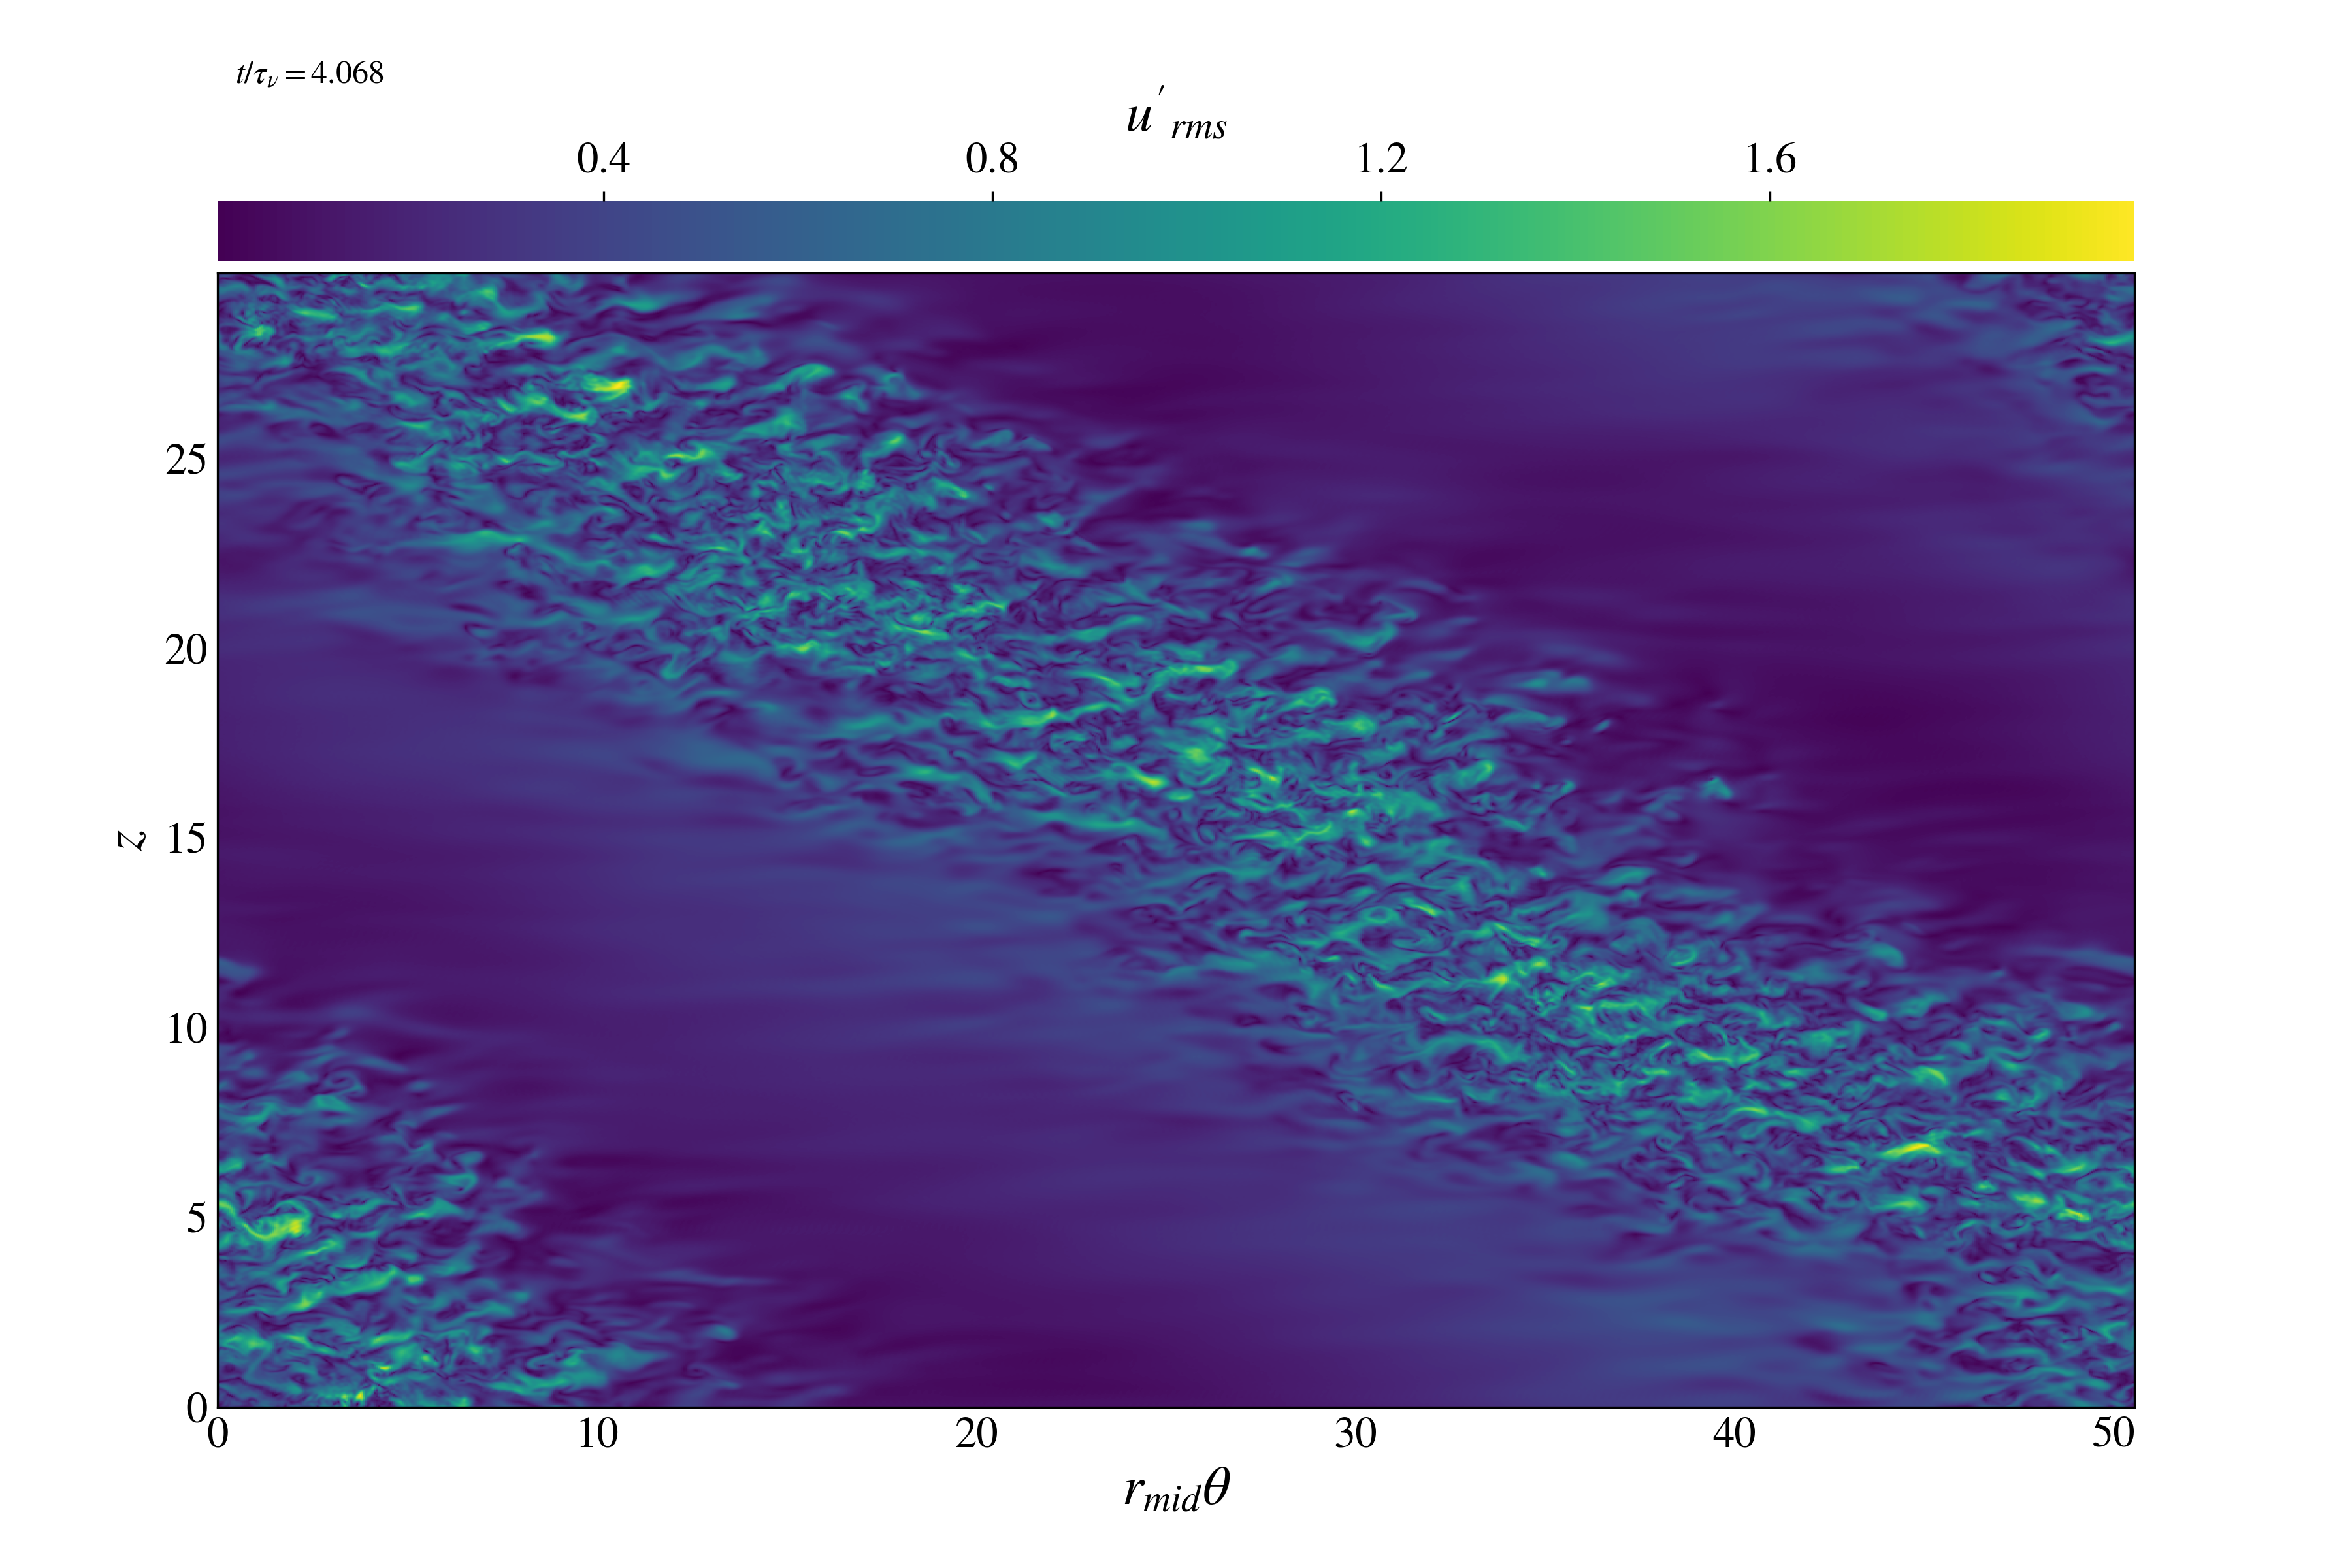
\includegraphics[width=\textwidth]{../figs/urms_tz_rei_700_reo-3398_000278.png}
    \caption{Slice of fluctuating rms velocity in the middle of the radial domain at $\Reyn_i = 700$, $\Reyn_o = -3398$. This solution is well below the linear stability threshold at }
    \label{fig:urms_tz_rei700}
\end{figure}
\subsection{Supercritical Spiral Turbulence}
We first consider the supercritical case with $\Reyn_i = 900$. We initialize GQL simulations with $\Lambda = 0, 1, 3, 5, 10$ using a snapshot of DNS data at $t \simeq 1.5 \tau_\nu$.  Figure~\ref{fig:rei900_snapshots} shows slices at mid-gap, $r = R_{mid}$. The first important thing to note is that none of these low-order models are able to maintain the spiral structure. However, even including a single additional low mode, $\Lambda = 1$, shows a significant improvement in flow morphology compared to QL. It is quite interesting to note that QL \emph{does} feature some degree of spatial intermittency--there are clearly separated regions hosting spiral waves interspersed with featureless, laminar patches. 
\begin{figure}
    \centering
    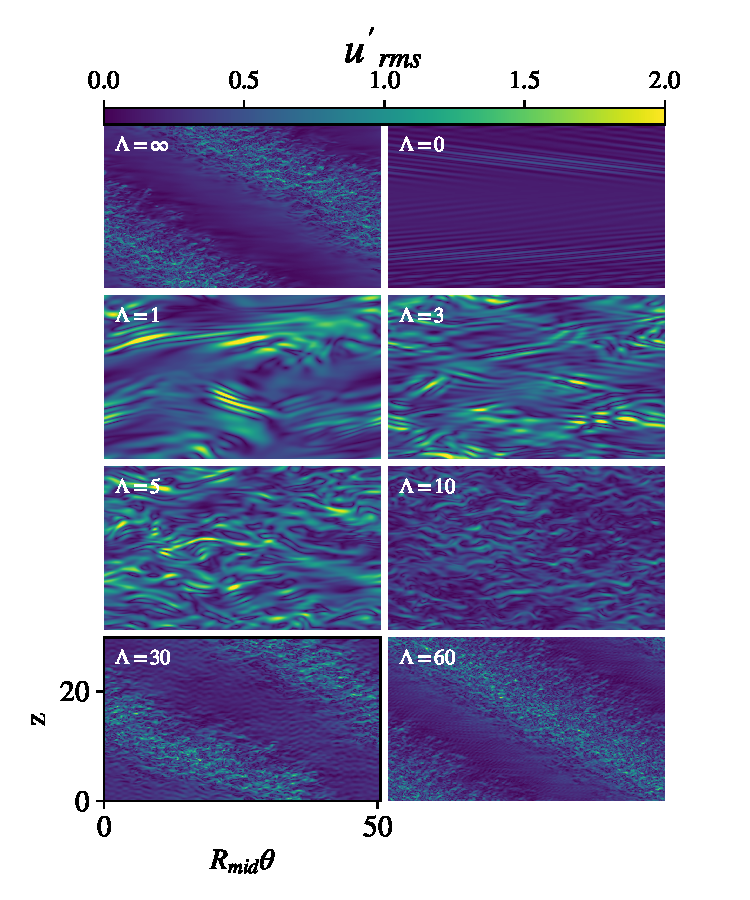
\includegraphics[width=\textwidth]{figs/rei900_snapshots.pdf}
    \caption{RMS velocity perturbations in the $z-\theta$ plane at $r=R_{mid}$ for $\Reyn_i=900, \Reyn_0=-3398$. The upper left panel shows DNS, the upper right panel shows QL, and the remaining four are GQL with $\Lambda = 1,3,5,10$. Even at $\Lambda = 10$, spiral turbulence is not apparent.}
    \label{fig:rei900_snapshots}
\end{figure}


Figure~\ref{fig:ke_vs_t_rei900} shows the kinetic energy as a function of time and $\Lambda$ for both the supercritical (left) and subcritical (right) runs. 
The supercritical case shows significant oscillations at all $\Lambda$. 
\begin{figure}
    \centering
    \begin{minipage}{0.45\textwidth}
        \centering
        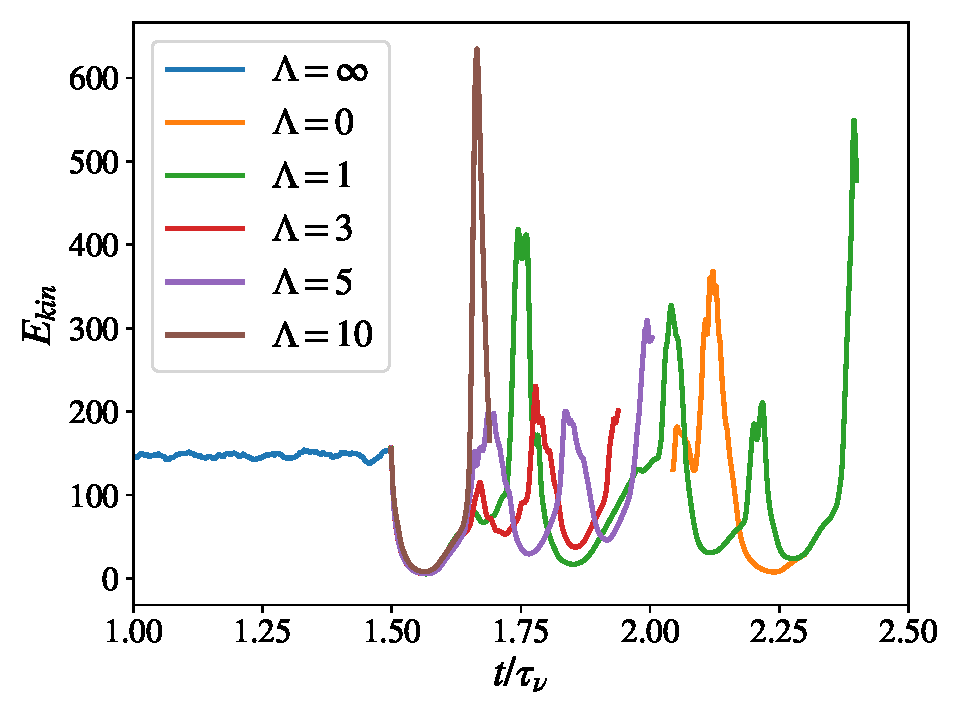
\includegraphics[width=0.9\textwidth]{figs/rei900_reo_-3398_KE_vs_t.pdf}
    \end{minipage}
    \begin{minipage}{0.45\textwidth}
        \centering
        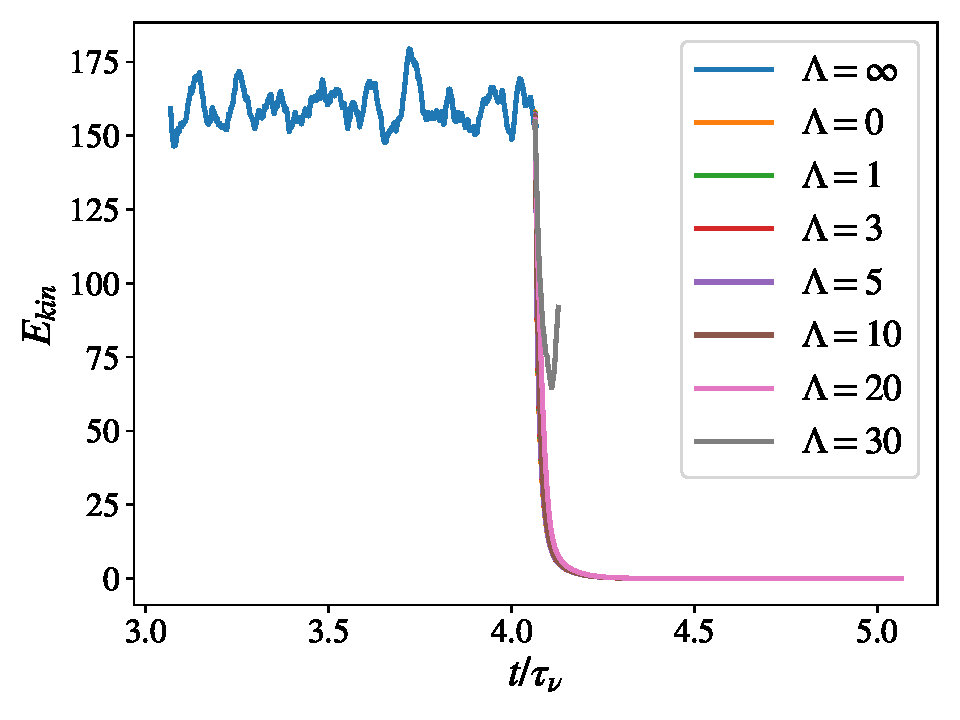
\includegraphics[width=0.9\textwidth]{figs/rei700_reo_-3398_KE_vs_t.pdf}
    \end{minipage}
    \caption{Perturbation kinetic energy as a function of time for $\Reyn_o=-3398$. On the left,  $\Reyn_i = 900$ is above the linear stability boundary, while the right shows $\Reyn_i = 700$, below the stability boundary. Starting from a saturated spiral turbulence state at $t/\tau_\nu \simeq 1.5$ (left), $t/\tau_\nu \simeq 3$ (right), we continue the solution with QL ($\Lambda = 0$) and GQL with cutoffs $\Lambda = 1,3,5,10$. For $\Reyn_i = 700$, we also use $\Lambda = 20, 30$ At higher $\Reyn_i$, all of the reduced models begin high amplitude oscillations. }
    \label{fig:ke_vs_t_rei900}
\end{figure}
Focusing on $\Lambda=5$, figure~\ref{fig:rei900_lambda5_story} shows that the flow goes through a series of different states bearing a strong resemblance to other well-known TC flow patterns originally identified in exhaustive series of experiments reported in \cite{1984JFM...146...45M} and subsequently found in simulations (e.g. \cite{2009PhRvE..80d6315M}). At the time of kinetic energy minimum, labelled 1 in the left hand side of figure~\ref{fig:rei900_lambda5_story}, the flow seems to recapitulate the interpenetrating spirals (IPS) characteristic of lower $\Reyn$ counter-rotating. As the kinetic energy rises, reaching a knee at point 2, the flow morphology resembles the patchy bursts characteristic of the intermittency regime (INT). Finally, at the peak of the kinetic energy oscillation, point 3 in figure~\ref{fig:rei900_lambda5_story}, the flow reaches is closests approach to something resembling spiral turbulence, though it is very difficult to identify the flow as such from a slice at a single point in time and plane in space.

This is notable for a few reasons. At $\Reyn_i=900, \Reyn_o=-3398$ the system is not in a hysteretic region of parameter space. Thus, we do not expect this behaviour to be due to GQL picking up other, coexisting solutions. 
It also highlights the delicate balance an intermittent laminar/turbulent solution represents. The turbulence in this solution has a very broad range of scales, as evidenced by figure~\ref{fig:urms_tz_rei700}. Understanding how it exchanges energy with the mean flow is crucial to understanding both the saturation of the underlying linear instability as well as the maintenance of the non-linear state. 
\begin{figure}
    \centering
    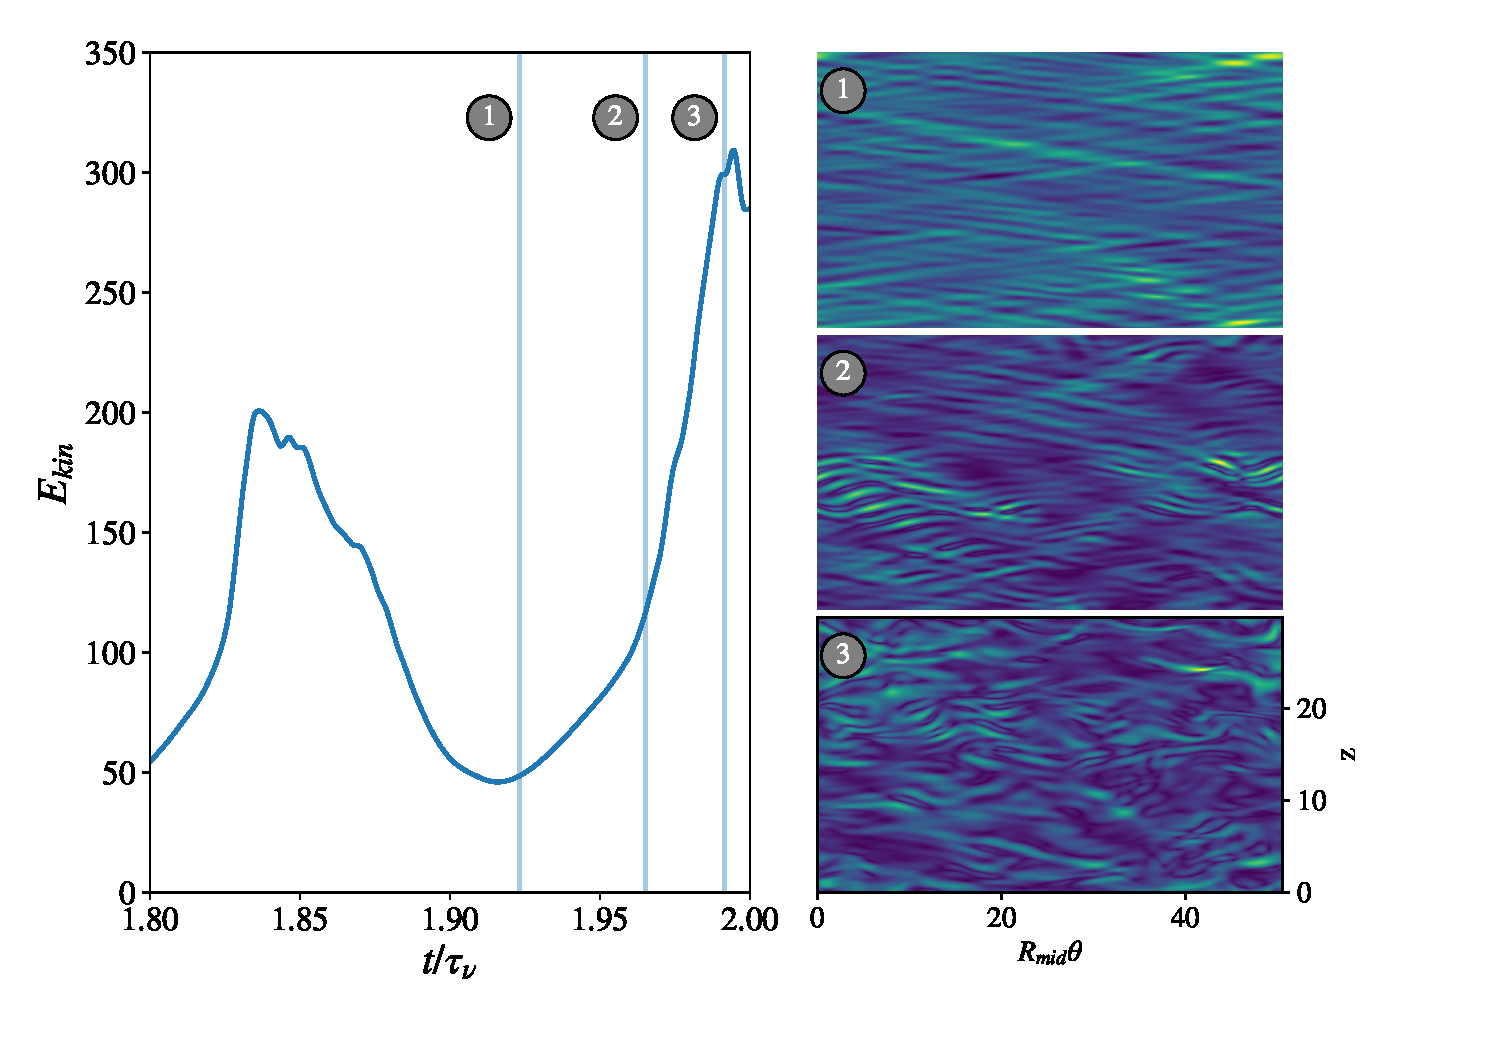
\includegraphics[width=0.9\textwidth]{figs/rei900_story.pdf}
    \caption{Kinetic energy (left) and flow morphologies (right) for $\Reyn_i = 900$, $\Lambda = 5$ covering one full oscillation cycle. The panels on the right show three times corresponding to the vertical lines in the kinetic energy plot on the left. At the kinetic energy minimum (point 1), the flow shows a IPS-like morphology, while an INT burst occurs at the knee (point 2), and a more space-filling turbulent state occurs at maximum energy (point 3).}
    \label{fig:rei900_lambda5_story}
\end{figure}

\begin{figure}
    \centering
    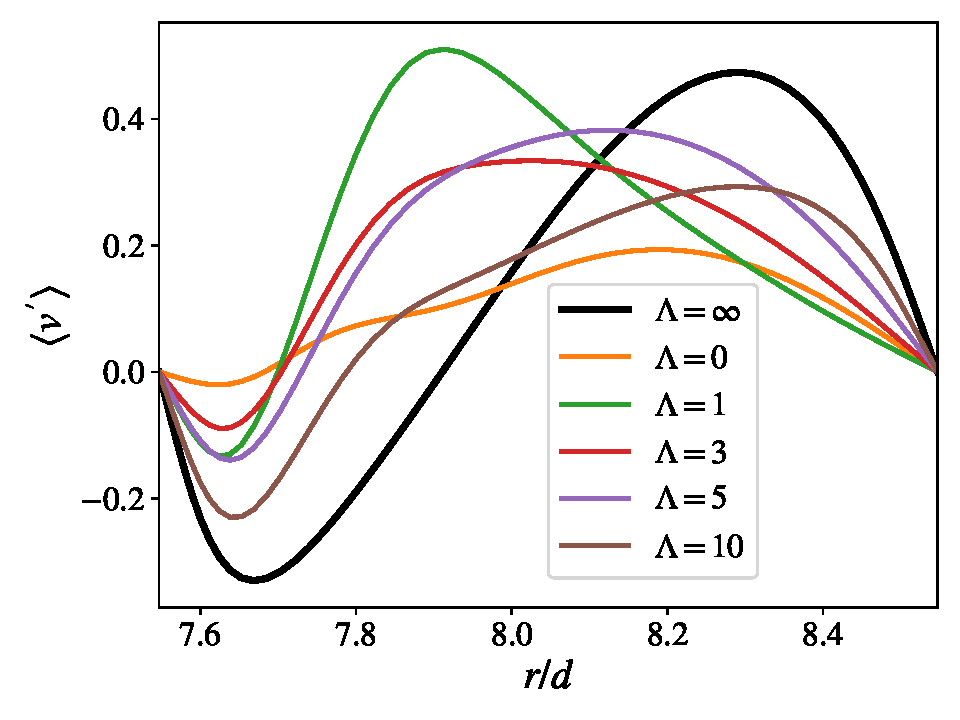
\includegraphics[width=0.9\textwidth]{figs/rei900_reo_-3398_vmean_profile.pdf}
    \caption{Mean deviation from CCF for $\Reyn_i = 900$, $\Reyn_o=-3398$. The heavy line is DNS, the orange line is QL, and all others are GQL with $\Lambda = 1,3,5,10$.}
    \label{fig:rei900_vmean}
\end{figure}

\subsection{Subcritical spiral turbulence}
In order to study subcritical spiral turbulence, we ran a series of DNS with decreasing $\Reyn_i$. Each is initialised with the last timestep of the prior run and run for one viscous time. Once we reached $\Reyn_i = 700$, we run a DNS for a final viscous time and then repeat the procedure from the supercritical GQL study. HThe right panel of figure~\ref{fig:ke_vs_t_rei900} shows  that all $\Lambda < 30$ revert to the laminar state within $0.1 \tau_\nu$. Our very preliminary data for $\Lambda = 30$ show that it recovers from the decay and begins to climb in energy again, similar to the early behaviour from the supercritical runs.\footnote{\textbf{Note to reviewers}: this simulation is still running as of the 31 July due date for the initial manuscript. By the time refereeing begins, we will update this plot and section.}

\section{Conclusion}
\label{sec:conclusion}
We have presented a series of simulations demonstrating the performance of GQL at various cutoffs for Taylor-Couette flow in the spiral turbulence regime. GQL is a significant improvement over QL models in representing mean quantities, including the deviation from circular Couette flow. However, even at the highest cutoffs studied here, it does not retain an unambiguous spiral form in either the sub- or supercritical regimes. Prior work has focused on the utility of GQL in presenting a more accurate \emph{statistical} picture of turbulent flows than QL \cite{2016PhRvL.116u4501M, 2017JFM...810..412T,2018RSPSA.47480422T,2019Kellam}. This focus is particularly important in light of its potential as as means of improving the accuracy of direct statistical simulation (DSS), a method for studying turbulence by computing its statistics directly, rather than individual realizations \cite{2022arXiv220505513M}. 

However, we have shown here that it is possible to use GQL as a means to investigate the non-linear interactions of greatest importance for maintaining the intricate patterns manifested in Taylor-Couette flow. In future work, we will consider the ability of GQL to maintain exact coherent states identified by Deguchi et al \cite{2014PhRvL.112r4502D} and the dynamics of which were studied recently by Wang and coworkers \cite{2022arXiv220712990W}. Understanding how these interactions work to shape subcritical TC turbulence represents a promising new avenue to understanding how ECS are maintained and how they in turn sustain turbulence below linear stability bounds. In particular, one can begin to understand the relative importance of 

\dataccess{All code for non-linear initial value problems, linear eigenvalue and non-modal stability analyses, and plotting are available at \url{https://github.com/jsoishi/GQL_TC}. Dedalus version 2 is available at \url{https://github.com/DedalusProject/dedalus/tree/v2_master}. eigentools is available at \url{https://github.com/DedalusProject/eigentools}. Simulation data is available upon request.}

\aucontribute{JSO wrote the manuscript, designed the study, wrote the GQL projection operators, and implemented the original Taylor-Couette Dedalus script. MB added the GQL terms to the TC script, developed data analysis techniques, and performed preliminary simulations.}

\competing{The authors declare that they have no competing interests.}

\funding{JSO was supported by NASA LWS grant number NNX16AC92G and NASA HTMS grant number 80NSSC20K1280. MB was supported in part by a Bates College Travel Grant.}

\ack{We thank Ben Brown for his help validating the Taylor-Couette code and John Mieszczanski for helping with resolution studies.  Computations for this paper were performed on the \emph{Leavitt} cluster at the Bates High Performance Computing Center and the NASA Pleiades system under allocation s2276.}

%%%%%%%%%% Insert bibliography here %%%%%%%%%%%%%%

\bibliographystyle{RS}
\bibliography{TC}
 
\end{document}
